% Template for Data Science Workshop 2018 paper; to be used with:
%          spconf.sty  - ICASSP/ICIP LaTeX style file, and
%          IEEEbib.bst - IEEE bibliography style file.
% --------------------------------------------------------------------------
\documentclass{article}
\usepackage{spconf,amsmath,graphicx}
\usepackage{array}
\usepackage{amsmath}
\usepackage{diagbox}

% Example definitions.
% --------------------
\newcommand{\X}{\mathbf{X}}
\newcommand{\Y}{\mathbf{Y}}
\newcommand{\oO}{\mathbf{O}}
\newcommand{\oOr}[1]{\mathbf{O}_{#1}}
%\newcommand{\Or}[1]{{O}^{(#1)}}
%\newcommand{\Ar}[1]{\mathcal{A}^{(#1)}}
%\newcommand{\oo}{\mathbf{o}}
%\newcommand{\oor}[1]{\mathbf{o}^{(#1)}}
\newcommand{\yr}[1]{y_{#1}}
\newcommand{\deltar}[1]{\delta_{#1}}
%\newcommand{\zr}[1]{z^{(#1)}}
\newcommand{\wW}{W}
%\newcommand{\wWr}[1]{W^{(#1)}}

\newcommand{\pr}{{P}}
\newcommand{\prhat}{\hat{\mathbb{P}}}
\newcommand{\sS}{S}

\newcommand{\pP}{\mathcal{P}}
\newcommand{\pPhat}{\hat{\mathcal{P}}}
\newcommand{\DL}{\mathcal{D_L}}
\newcommand{\DU}{\mathcal{D_U}}
\newcommand{\lat}{\mathcal{L}}
\newcommand{\latr}[1]{\lat^{(#1)}}

\newcommand{\DenG}{\mathcal{G}_\text{DEN}}
\newcommand{\NumG}{\mathcal{G}_\text{NUM}}

%\newcommand{\NumPost}[1]{\gamma_t^{(r)NUM}(j;#1)}
\newcommand{\NumPost}[1]{\gamma_{rt}^{NUM}(j;#1)}
\newcommand{\DenPost}[1]{\gamma_{rt}^{DEN}(j;#1)}

\newcommand{\Fkl}{\mathcal{F}_\text{KL}}
\newcommand{\Fmmi}{\mathcal{F}_\text{MMI}}

\newcolumntype{C}[1]{>{\centering\arraybackslash\hspace{0pt}}p{#1}}
\newcolumntype{R}[1]{>{\raggedleft\arraybackslash\hspace{0pt}}p{#1}}
\newcolumntype{L}[1]{>{\raggedright\arraybackslash\hspace{0pt}}p{#1}}


% Title.
% ------
\title{A teacher-student learning approach for unsupervised domain adaptation of sequence-trained ASR models}
%
% Single address.
% ---------------
\name{Vimal Manohar$^{1,2}$, Pegah Ghahremani$^1$, Daniel Povey$^{1,2}$, Sanjeev
Khudanpur$^{1,2}$
\thanks{This work was partially supported by NSF Grant No CRI-1513128 and
IARPA MATERIAL award number FA8650-17-C-9115.}}
\address{
  $^1$Center for Language and Speech Processing\\
  $^2$Human Language Technology Center Of Excellence\\
  Johns Hopkins University, Baltimore, MD 21218 \\
  \texttt{\{vimal.manohar91,pegahgh,dpovey\}@gmail.com,khudanpur@jhu.edu}}
%
% For example:
% ------------
%\address{School\\
%	Department\\
%	Address}
%
% Two addresses (uncomment and modify for two-address case).
% ----------------------------------------------------------
%\twoauthors
%  {A. Author-one, B. Author-two\sthanks{Thanks to XYZ agency for funding.}}
%	{School A-B\\
%	Department A-B\\
%	Address A-B}
%  {C. Author-three, D. Author-four\sthanks{The fourth author performed the work
%	while at ...}}
%	{School C-D\\
%	Department C-D\\
%	Address C-D}
%
\begin{document}
%\ninept
%
\maketitle
%
\begin{abstract}
Teacher-student (T-S) learning is a transfer learning approach, where a teacher 
network is used to ``teach'' a student network to make the
same predictions as the teacher. Originally formulated for model compression,
this approach has also been used for domain adaptation, and is particularly
effective when parallel data is available in source and target domains.
The standard approach uses a frame-level objective of minimizing the KL
divergence between the frame-level posteriors of the teacher
and student networks. However, for sequence-trained models for speech
recognition, it is more appropriate to train the student to mimic the
sequence-level posterior of the teacher network. In this work, we compare this
sequence-level KL divergence objective with another semi-supervised
sequence-training method, namely the lattice-free MMI, for unsupervised
domain adaptation. We investigate the approaches in multiple scenarios
including adapting from clean to noisy speech, bandwidth mismatch and
channel mismatch.
\end{abstract}
%
\begin{keywords}
sequence training, lattice-free, transfer learning, unsupervised adaptation,
automatic speech recognition
\end{keywords}
%
\section{Introduction}
\label{sec:intro}

Transfer learning is the general machine learning approach of transferring
knowledge from one model to another. Depending on the context it is used in,
it might be called different things.
In the case where we have to learn
a smaller model on the same domain, the approach is called ``model
compression''.
In the case, where we have to learn a model
in a different domain, the approach is called ``domain adaptation''.
There is a rich survey of transfer learning methods in the
literature \cite{pan2010survey,lu2015transfer,bengio2012deep}.
Transfer learning methods have been applied to speech processing in various
settings. Wang et. al \cite{wang2015transfer} gives a good overall survey of
methods used in speech processing.

Sequence discriminative training, e.g. using Maximum Mutual Information (MMI)
\cite{bahl-mmie},
has been shown to improve performance of frame-level cross-entropy trained
neural networks. Of late, neural networks are trained from scratch
using sequence objectives like Connectionist Temporal Classification (CTC)
\cite{graves2006ctc} and Lattice-free MMI (LF-MMI)
\cite{chain}, and these usually out-perform the frame-level trained ones.
LF-MMI training has been investigated for supervised domain adaptation
\cite{pegah2017transfer} and semi-supervised training \cite{manohar2018semisup}.
Semi-supervised training methods like in \cite{manohar2018semisup} can also
be applied when the unsupervised data is from a slightly different domain than
the supervised data used to train the seed network. 
This was investigated for
speaker adaptation in \cite{kanda2017sequence-kl} using 1-best hypotheses 
from decoding.
% * <pegahgh@gmail.com> 2018-06-29T20:14:11.350Z:
% 
% It can be written in better way. It is a bit wage. You may need to add citation
% 
% ^.
In this paper, we investigate this idea of using semi-supervised LF-MMI with
lattice-based supervision for unsupervised domain adaptation.

One of the methods for transfer learning is the teacher-student (T-S) approach
where a teacher network is used to ``teach'' a student network to make the 
same predictions as the teacher. It is traditionally used for model compression
\cite{bucilua2006model} as in \cite{ba2014deep,hinton2015distilling}. It has also
been applied in context of domain adaptation \cite{yu2013kl}, where the teacher
network is trained on the source domain and the student network is trained on
the target domain. It is particularly effective when parallel data is available
in source and target domains \cite{li-2017-teacher-student}. Here, a large 
amount of unsupervised data in parallel source and target domains is used to 
improve performance of the model on target domain. However, these works do 
not compare with standard semi-supervised training methods that can also be used
to do unsupervised adaptation. One of the goals of this work is to 
compare T-S learning objective with a standard semi-supervised training
approach like using LF-MMI.

The standard approach for T-S learning uses an objective of minimizing 
the KL divergence between the frame-level posteriors of the teacher and student
networks. However, this may not be applicable to state-of-the-art 
speech recognition models that are trained at the sequence-level, and in
particular using LF-MMI. Alternatively, in this work, we use the 
KL divergence between sequence-level posteriors
\cite{wong2016sequence-ts,kanda2017sequence-kl} 
from the teacher and student networks as the training objective. The similarity
of this objective to LF-MMI allows it to be integrated easily into the
lattice-free training framework.

In this paper, we investigate two sequence objectives for
teacher-student type transfer learning for unsupervised adaptation --
semi-supervised LF-MMI and sequence-level KL divergence.
We describe our methods in Section \ref{sec:proposed-method}. 
In Section \ref{sec:experiments}, we describe
experiments to evaluate our proposed method in the scenario of domain adaptation.
We look at three scenario for adaptation -- clean to noisy speech, 8kHz to 16kHz
audio, and headset microphone to distant microphone.
Finally, in Section \ref{sec:conclusions}, we present conclusions and future
work.

\section{Related works}

A sequence-KL objective for T-S learning was introduced in
\cite{wong2016sequence-ts} for model compression from an ensemble. 
Unlike that work which used lattice-based discriminative training, here we apply
sequence-level KL divergence in the lattice-free training framework for 
unsupervised domain adaptation. 
In \cite{kanda2017sequence-kl}, a lattice-free
sequence-KL objective was introduced for model compression
and speaker adaptation.
Our work in this paper differs in how the supervision for training the student
is generated. In particular, we propose a simpler way to get the supervision
using the lattice supervision approach used for semi-supervised LF-MMI training 
in \cite{manohar2018semisup}. We also investigate
the effect of using different LMs both when creating the numerator supervision 
and the denominator graph.

KL divergence objective is also viewed as a regularizer, which prevents the
model from diverging too much from what the original model predicts
\cite{yu2013kl}. A sequence-level KL version of this idea was used to regularize
LF-MMI based DNN adaptation in \cite{long2017domain,kanda2017sequence-kl} to
small adaptation sets.
On the other hand, our work in this paper focuses on unsupervised domain
adaptation when we have large unsupervised target-domain dataset. We also train 
our neural networks from scratch since the input features to the student 
network might be different from that of the teacher network (e.g. 16kHz vs
8kHz).
In this context, we can view
the sequence-level KL objective to be regularizing semi-supervised LF-MMI
training to prevent to the model from over-fitting to the unsupervised data.


\section{Proposed methods}
\label{sec:proposed-method}

%In the following sections, we describe our proposed
%sequence training methods -- Semi-supervised LF-MMI (Section \ref{sec:lfmmi}) 
%and sequence-KL divergence (Section \ref{sec:seq-kl}). Then in Section
%\ref{sec:compare-mmi-kl}, we compare the two objectives. 
%In Section \ref{sec:combine-mmi-kl},
%we describe how we can combine the two objectives for training.

\subsection{Semi-supervised Lattice-free MMI}
\label{sec:lfmmi}

Semi-supervised LF-MMI training was proposed in \cite{manohar2018semisup}.
Here, we extend that work to the scenario of domain adaptation when there is 
parallel unsupervised data in source and target domains.
In \cite{manohar2018semisup}, a seed network trained on the supervised data 
is used to decode the unsupervised data to generate lattices containing the
hypothesized phone sequences.
The lattices are converted into numerator graphs (denoted $\NumG$) using the 
smart-splitting method described in \cite{manohar2018semisup} and 
composing with a
normalization FST \cite{chain} whereby we interpolate the word 
LM scores from the lattice and phone LM scores from the denominator graph 
$\DenG$. The LF-MMI objective is:
\begin{align}
	\Fmmi =& \sum_r \log \sum_{\pi\in\NumG} 
  \pr(\pi\mid \oOr{r}) \\
  =& \sum_r \log \frac{\sum_{\pi\in\NumG} \pr(\oOr{r}\mid\pi) \pr(\pi)} {\pr(\oOr{r})}
  \label{eq:lfmmi}
\end{align}
where $\oOr{r}$ is the sequence of acoustic observations for utterance $r$, 
$\pi$ is a HMM state sequence in the numerator graph $\NumG$ or
denominator graph $\DenG$ and the likelihood
$\pr(\oOr{r}) \approx \sum_{\pi\in\DenG} \pr(\oOr{r}\mid\pi) \pr(\pi)$.
We extend this trivially for domain adaptation. Here, a seed network 
(referred to as the teacher model) is trained on the supervised data from the
source domain. This is used to decode the unsupervised data in the source domain
to generate lattices containing the hypothesized state sequences.  These
lattices are also the hypotheses for the corresponding parallel data in the
target domain. 
So they are converted into supervision for training the student model in the 
target domain. The student model is trained with this as the supervision and 
the parallel target domain data as input. Such a use of parallel data for LF-MMI
training was also found to be useful for far-field ASR in \cite{vijay_ami}.

\subsection{Sequence-KL objective}
\label{sec:seq-kl}

Sequence-KL objective was proposed for T-S learning
in \cite{wong2016sequence-ts}. The objective here is to make the student network
mimic the teacher network by maximizing the 
negative KL divergence between sequence-level posteriors from the teacher and 
student networks as shown in \eqref{eq:lattice-free-kl}. 
We describe in this section our implementation in the lattice-free training
framework and how it differs from those in other similar works in
\cite{wong2016sequence-ts,kanda2017sequence-kl}.
%Later in Section \ref{sec:experiments}, we show experimental 
%results comparing the various methods for getting the supervision for training
%with this objective. 

\begin{align}
  \Fkl =& -\sum_r \sum_{\pi\in\NumG} \pr(\pi\mid \oOr{r}; \lambda^*) 
  %\F =& -\sum_r \sum_{\pi\in\lat} \pr(\pi\mid \oOr{r}; \lambda^*) 
  \log\left[\frac{\pr(\pi\mid \oOr{r}; \lambda^*)}{\pr(\pi\mid \oOr{r};
  \lambda)}\right], \label{eq:lattice-free-kl} \\
  %\propto& \sum_r \sum_{\pi\in\lat} \pr(\pi\mid \oOr{r};
  %\lambda^*)\log\pr(\pi\mid \oOr{r}; \lambda) \nonumber \\
  %=& \sum_r \sum_{\pi\in\lat} \pr(\pi\mid \oOr{r}; \lambda^*)\log 
  %\left[\pr(\oOr{r}\mid \pi; \lambda)\pr(\pi)\right] \nonumber \\ 
  %& - \log \pr(\oOr{r}; \lambda) \nonumber \\
  \propto& \sum_r \biggl(\sum_{\pi\in\NumG} \pr(\pi\mid \oOr{r}; \lambda^*)\log 
  \pr(\oOr{r}\mid \pi; \lambda) \nonumber \\
  & - \log \pr(\oOr{r}; \lambda) \biggr),\label{eq:kl-simplified}
\end{align}
where 
$\pr(\pi\mid \oOr{r}; \lambda^*)$ and
$\pr(\pi\mid \oOr{r}; \lambda)$ are posterior probabilities of 
the HMM state sequence $\pi$ obtained from the teacher network (parameterized by
$\lambda^*$) and the student network (parametrized by $\lambda$) respectively.
The former quantity is a constant since the teacher network is
fixed when training the student. The simplification\footnote{using Bayes rule and removing 
  the constant additive terms. Also $\sum_{\pi\in\NumG} \pr(\pi\mid \oOr{r};
\lambda^*)=1$} to \eqref{eq:kl-simplified} 
makes it clear that the objective
consists of numerator and denominator terms.

\subsubsection{Denominator term}
The denominator term $\log \pr(\oOr{r}; \lambda)$ 
i.e. the log-likelihood under the student network is independent of 
the teacher network. 
In \cite{wong2016sequence-ts}, this term
was computed using a denominator lattice generated using a unigram LM. 
However, in lattice-free training, we compute this over a 
fixed denominator graph, $\DenG$, just as in the case of LF-MMI. 
The reader is directed to \cite{chain}
for details of this forward-backward \cite{rabiner1989tutorial} computation on a GPU.
As in \cite{chain}, the denominator graph is created using a 4-gram phone LM. 
To bias it to the target domain, we use interpolated counts from source and
target domains as in \cite{vimal2017mgb3}.

\subsubsection{Numerator term}
We compute the first term in \eqref{eq:kl-simplified} i.e. the numerator term 
as a summation over HMM
state sequences $\pi=s_1\dots s_T$ in the numerator graph $\NumG$ created by
decoding the utterance using the teacher network. This is the same
numerator graph that is generated for the semi-supervised LF-MMI 
training described in Section \ref{sec:lfmmi}. This is also where we
differ from \cite{kanda2017sequence-kl}. In \cite{kanda2017sequence-kl}, 
this summation is done over the weak denominator graph $\DenG$.
However, we are doing this summation over a lattice-based 
supervision that is generated using a strong 3-gram or 4-gram word LM. 
Our results in Section \ref{sec:experiments} show that using a strong LM here
is generally better. This is also easier to implement since the lattice-based 
supervision is already generated for semi-supervised LF-MMI training. 

\subsubsection{Derivative computation}
Since teacher network is fixed, the derivative of $\Fkl$ w.r.t.
the student network output of utterance $r$ at time $t$, $\yr{rt}(j;\lambda)$, is:
\begin{alignat}{2}
 \frac{\partial\Fkl}{\partial \yr{rt}(j;\lambda)} %=& \sum_{\pi\in\lat} \pr(\pi\mid\oOr{r};
 %\lambda^*) \delta(s_t(\pi)=j) -\gamma_t^{(r)DEN}(j;\lambda) \nonumber \\
 =& \NumPost{\lambda^*} - \DenPost{\lambda}, \label{eq:kl-deriv} 
\end{alignat}
where 
$\NumPost{\lambda^*}$, the numerator posterior, is
the posterior probability of senone $j$ at time $t$ computed over the
numerator graph $\NumG$ using the teacher network and 
$\DenPost{\lambda}$, the denominator posterior, 
is the posterior probability of senone $j$ at time $t$ computed over
the denominator graph $\DenG$ using the student network.
These are computed as:

\begin{alignat}{2}
  \NumPost{\lambda^*} &= \frac{\sum_{\pi\in\NumG}
  \deltar{rt}(j) \pr(\oOr{r}\mid \pi; \lambda^*) \pr(\pi)} {\sum_{\pi'\in\NumG}
  \pr(\oOr{r}\mid \pi'; \lambda^*) \pr(\pi')}, \label{eq:num-post} \\
  \DenPost{\lambda} &= \frac{\sum_{\pi\in\DenG}
  \deltar{rt}(j) \pr(\oOr{r}\mid \pi; \lambda) \pr(\pi)} {\sum_{\pi'\in\DenG}
  \pr(\oOr{r}\mid \pi'; \lambda) \pr(\pi')}, \label{eq:den-post}
\end{alignat}
where $\deltar{rt}(j)$ is 1 iff HMM state $s_t$ in sequence $\pi$ corresponds
to senone $j$ and 0 otherwise. Both the numerator and denominator posteriors
are computed over their respective graphs using forward-backward algorithm
\cite{rabiner1989tutorial}. Further, since the teacher network is fixed, these numerator posteriors can be precomputed and dumped to the disk. 

%Since the teacher network parameters are fixed, the 
%numerator term decomposes over the context-dependent states (senones or p.d.f. 
%in Kaldi terminology) in the HMM:
%
%\begin{equation}
%  \begin{aligned}
%    \sum_{\pi\in\NumG} \pr(\pi\mid \oOr{r}; \lambda^*)\log 
%    \pr(\oOr{r}\mid \pi; \lambda) \\ 
%    = \sum_t \sum_j \gamma_t^{(r)NUM}(j;\lambda^*) y_t^{(r)}(j;\lambda),
%    \label{eq:kl-num}
%  \end{aligned}
%\end{equation}
%
%where $y_t^{(r)}(j;\lambda) = \log p(o_t\mid j; \lambda)$ is the log-likelihood
%of senone $j$ at time
%$t$ under the student network\footnote{Unlike the cross-entropy trained 
%  neural networks that output posteriors, here, we are training the 
%  student network to directly output log-likelihoods just as we do for LF-MMI
%  training. The reader is directed to \cite{chain} for details.} 
%and $\gamma_t^{(r)NUM}(j;\lambda^*)$ (referred to as the numerator posterior) is
%the posterior probability under the teacher network of senone $j$ at time $t$ 
%computed over the numerator graph $\NumG$.
%\footnote{ $\gamma_t^{(r)NUM}(j;\lambda^*) = \frac{\sum_{\pi\in\NumG}
%  \delta_{jt}^{(r)} \pr(\oOr{r}\mid \pi; \lambda^*) \pr(\pi)} {\sum_{\pi'\in\NumG}
%\pr(\oOr{r}\mid \pi'; \lambda^*) \pr(\pi')} $}
%The numerator term and numerator posteriors 
%are both computed using a forward-backward algorithm \cite{rabiner1989tutorial} 
%over the numerator graph.

%%Using \eqref{eq:kl-simplified} and \eqref{eq:kl-num}, it is easy to see that the
%%derivative of the sequence-KL objective function w.r.t. to the $j^\mathrm{th}$
%%senone output of the network at time $t$ is as in:
%%
%%\begin{alignat}{2}
%% \frac{\partial\Fkl}{\partial \yr{rt}(j;\lambda)} %=& \sum_{\pi\in\lat} \pr(\pi\mid\oOr{r};
%% %\lambda^*) \delta(s_t(\pi)=j) -\gamma_t^{(r)DEN}(j;\lambda) \nonumber \\
%% =& \gamma_t^{(r)NUM}(j;\lambda^*) -\gamma_t^{(r)DEN}(j;\lambda), \label{eq:kl-deriv} 
%%\end{alignat}
%%where 
%%$\gamma_t^{(r)NUM}(j;\lambda^*)$ is the numerator posterior from teacher
%%network as described in the previous section
%%%posterior probability of senone
%%%$j$ at time $t$ under the teacher network computed over the numerator graph $\NumG$
%%%and 
%%$\gamma_t^{(r)DEN}(j;\lambda)$ is the posterior probability of senone
%%$j$ at time $t$ under the student network computed over the denominator graph
%%$\DenG$.
%%
%%As can be seen in \eqref{eq:kl-deriv}, the derivative is the difference of the 
%%numerator posterior from the teacher network and the denominator posterior from
%%the student network.
%%The difference is that in MMI, the first term in the derivative is the numerator
%%posterior from the student network, also computed over the same supervision
%%graph $\NumG$.

\subsubsection{Lattice-free MMI and sequence-KL}
\label{sec:combine-mmi-kl}

From \eqref{eq:kl-deriv}, we can see that the derivative is the
difference of the numerator posterior computed using the {\em teacher network} 
and the denominator posterior computed using the student network. Note that 
this differs only in the first term from the derivative of the MMI objective
\eqref{eq:lfmmi}:
\begin{alignat}{2}
 \frac{\partial\Fmmi}{\partial \yr{rt}(j;\lambda)} %=& \sum_{\pi\in\lat} \pr(\pi\mid\oOr{r};
 %\lambda^*) \delta(s_t(\pi)=j) -\gamma_t^{(r)DEN}(j;\lambda) \nonumber \\
 =& \NumPost{\lambda} - \DenPost{\lambda}, \label{eq:mmi-deriv} 
\end{alignat}
where the first term is the numerator posterior computed using the {\em student
network} i.e. with $\lambda$ instead of $\lambda^*$ in \eqref{eq:num-post}. 
%Note that this computation is done in each minibatch of training the student network. 

To use an interpolation of the two objectives, we can simply interpolate the 
numerator posteriors from teacher and student networks. This is a 
sequence-level analogue to the knowledge distillation idea
\cite{hinton2015distilling}, and this was also explored in
\cite{kanda2018sequence-kl}. In our work, we always 
compute the numerator of the LF-MMI objective using a supervision lattice 
generated using a strong 3-gram word LM. But in Section 
\ref{sec:experiments}, we explore computing the numerator of the sequence-KL
objective using a different supervision lattice such as one generated using
a weak LM like a unigram LM.

%One distinction between the supervision used for sequence-KL 
%and that used for LF-MMI is that the former uses a frame tolerance of 0.
%In \cite{manohar2018semisup}, frame tolerance of $\pm30ms$ was used for LF-MMI
%to allow senones to appear slightly ahead or behind where they appeared in
%the lattice. For sequence-KL, we had to force the senones to appear
%exactly where they did in the lattice. The reason for this is that if we used a
%higher frame tolerance, we would have to recompute the acoustic scores in
%the supervision by propagating through the teacher network. 
%% * <pegahgh@gmail.com> 2018-06-29T20:52:13.355Z:
%% 
%% I think they don't understand these details. It is better to describe simpler or with figure or formultation
%% 
%% ^.
%But for a frame tolerance of 0, we can simply use the existing acoustic
%scores in the lattice and dump the numerator posteriors.

\section{Experiments}
\label{sec:experiments}

We compare semi-supervised LF-MMI and sequence-level KL divergence 
for domain adaptation in the following scenario -- Clean to noisy speech, 8kHz
Fisher to 16kHz AMI, and headset microphone to distant microphone speech. 

All the neural networks in our experiments have an architecture with time-delay
neural network (TDNN) \cite{tdnn,vijay-tdnn} layers interleaved with LSTM
\cite{sak2014lstmp} layers. We use per-frame dropout on the LSTM layers
\cite{cheng2017dropout}. The reader is directed to \cite{cheng2017dropout} 
for training details.  The scripts and code used for these experiments can be
found in a personal Kaldi
branch\footnote{https://github.com/vimalmanohar/kaldi/tree/semisup-ts}.
To avoid over-fitting, we apply the regularization methods suggested 
in \cite{chain} for both LF-MMI and sequence-KL training.
We use online i-vectors
\cite{karafiat-2011-ivector-adaptation,dehak2011ivectors,vijay_aspire} for
speaker adaptation. The teacher and the student networks use i-vectors extracted
from different i-vector extractors trained on their respective domains. Our
method for creating supervision is described in sections \ref{sec:lfmmi} and 
\ref{sec:seq-kl}. In some of the experiments, we use a semi-supervised style 
training where the supervised training uses LF-MMI objective computed on
lattices generated by force-aligning the word transcription using a HMM-GMM
system and the unsupervised training uses LF-MMI or sequence-KL objective
computed on lattices generated by decoding as described in Section
\ref{sec:lfmmi}. 

\subsection{Clean to noisy speech}
\label{sec:aspire_expts}

In this section, we report results of unsupervised adaptation from
clean to noisy speech on Aspire corpus \cite{aspire}. 
The training data consists of 
1500 hours of Fisher English \cite{fisher-corpus}. 
Of this, we use 300 hours as 
supervised data with transcription and 1200 hours without transcription.
% * <pegahgh@gmail.com> 2018-06-29T20:57:48.535Z:
% 
% They may say that we  did that randomly and you should do leave-one-out cross-validation! 
% 
% ^.
The ``Baseline'' system is trained with LF-MMI objective on 300 hours supervised
data augmented 3x with reverberation and noise \cite{ko2017augmentation} and 3x
with speed and volume perturbation \cite{ko2015audio} (Hence 9x300 hours).
%% [Pegah] Do you mean that we have 3 + 3 = 6 x original data or 3 * 3 = 9 x original data?
The ``Oracle'' system is trained with LF-MMI objective using as supervised data
all 1500 hours augmented 3x with reverberation and noise. We use the same
i-vector extractor for baseline, oracle and all the student networks. This is
trained on 1500 hours of Fisher data augmented 3x with reverberation and noise.
% * <pegahgh@gmail.com> 2018-06-29T21:12:04.046Z:
% 
% So do you mean  that it is 4500 hrs after augmentation?
% 
% ^ <vimal.manohar91@gmail.com> 2018-06-30T23:11:25.510Z:
% 
% Yes
%
% ^.
% * <pegahgh@gmail.com> 2018-06-29T20:59:31.870Z:
% 
% I am not sure, but you described earlier that iVector extractor is trained on respective domain
% 
% ^ <vimal.manohar91@gmail.com> 2018-06-30T23:14:25.437Z:
% 
% Yes, this is all for the target domain.
%
% ^.

The teacher network is trained on ``clean" 300 hours supervised data with 
only 3x speed perturbation, but with no reverberation or noise addition.
This network is used to decode the whole 1500 
hours\footnote{Note that this includes the 300 hours of 
audio from supervised dataset, but we are only using the audio and not the 
transcripts. This is like using soft posteriors for labeled data in
conventional T-S learning~\cite{hinton2015distilling}.} 
of ``clean''
Fisher data. For this decoding, we use a 3-gram LM
trained on transcripts from the 300 hours supervised set.
We create the supervision for training the student network as described 
in Section \ref{sec:lfmmi} with 1500 hours of reverberated and noise corrupted
data (augmented 3x) parallel to the ``clean'' data. 
The denominator graph is generated using 4-gram phone LM created by averaging 
counts from supervised data alignments and 1-best alignments from
unsupervised data. We additionally interpolate the phone LM scores with the 
word LM scores in the lattice with a scale of 0.5 as found to be 
optimum in \cite{manohar2018semisup}.
% Pegah: Interesting, how much improvement did you get from scale 0.5? I expect that 300hrs supervised data should be enough to train consistent 4-gram LM for denom.
% * <pegahgh@gmail.com> 2018-06-29T21:14:00.995Z:
% 
% Do you have any results how much it improves the results? also why unweighted averaging?
% 
% ^.
The supervised training uses LF-MMI with supervision from a GMM system, while 
the unsupervised training uses an interpolated objective
$(1-\beta)\Fmmi+\beta\Fkl$. The $\beta$ used in each experiment is shown in 
Table \ref{tab:aspire_results}.
The columns ``sup'' and ``unsup'' show the amount of supervised and unsupervised 
data (prior to augmentation) respectively used in training the student network. 
The results in Table \ref{tab:aspire_results} show WER(\%) on 
{\em dev} and {\em test} sets, which are 3 hour subsets heldout from the 
Fisher English corpus, but reverberated and corrupted with noise. 
These are part of Kaldi \cite{kaldi_paper} Aspire recipe. We also report results 
on the official {\em aspire} development set~\cite{aspire}. 

%Pegah: We show that KL is better than LF-MMI. What about using MMI and initializing network with teacher? Did you use different network? I didn't find any network topology description for teacher and student.
% Pegah: It is interesting that we get improvement from row 2 to 4. Is 300 hrs supervised a subset of 1500 unsup data? If yes, I expected that posterior from teacher works like soft label for this data and I expect the results to be as good as using hard labels. 
From rows 2 and 3 showing results from training {\bf only} on the 
unsupervised data, we see that sequence-KL is significantly better than using 
LF-MMI. The WER with LF-MMI is worse than even the baseline on the {\em aspire} set.
But with semi-supervised training by including supervised data in a 
multitask approach \cite{manohar2018semisup} (Rows 4-6), 
we always get significant improvement over the baseline.
Further, using either sequence-KL (Row 5) or an interpolation of LF-MMI and 
sequence-KL (Row 6) is slightly better than using LF-MMI (Row 3). 
We then tried to use a unigram LM instead of a 3-gram LM for decoding when
generating numerator posteriors for the sequence-KL objective, 
while still using 3-gram for generating 
lattices for MMI training. From the row 7 in Table \ref{tab:aspire_results}, 
we see that this does not work as well. Since, it is easier to do decoding 
just once, we recommend just using the 3-gram LM for generated lattices for both
MMI and sequence-KL training.
%% Pegah: I am not sure, why did you add last row using posterior generated using unigram LM? Do you want to show the power of LM in KL training?
\begin{table}[t]
  \centering
  \caption{\label{tab:aspire_results} 
  WER(\%) results for unsupervised adaptation from clean to noisy.
  The objective is $(1-\beta) \Fmmi + \beta \Fkl$.}
  \begin{tabular}{lc|r r|ccc}
    System & $\beta$ & \multicolumn{2}{c|}{hrs} & \multicolumn{3}{c}{WER(\%)}
    \\
    & & sup & unsup & {\em dev} & {\em test} & {\em aspire} \\
    \hline
    \hline
    Baseline & 0.0 & 300 & 0 & 23.6 & 22.5 & 26.6 \\
    \hline
    Unsup & 0.0 & 0 & 1500& 23.0 & 22.0 & 27.0 \\
    Unsup & 1.0 & 0 & 1500& 21.8 & 21.0 & 25.9 \\
    \hline
    Semisup & 0.0 & 300 & 1500 & 21.6 & 21.0 & 25.1 \\
    Semisup & 1.0 & 300 & 1500 & 21.0 & 20.3 & 24.4 \\
    Semisup & 0.5 & 300 & 1500 & \bf 21.0 & \bf 20.2 & \bf 24.2 \\
    \multicolumn{1}{r}{+ UG} & 0.5 & 300 & 1500 & 21.2 & 20.6 & 24.5 \\
    \hline
    Oracle & 0.0 & 1500 & 0 & 19.1 & 18.4 & 23.3 \\
    \hline
  \end{tabular}
\end{table}

\subsection{8kHz Fisher to 16kHz AMI}
\label{sec:fisher_ami_expts}

In this section, we report results for domain adaptation from 8kHz Fisher 
to 16kHz AMI \cite{ami-corpus} individual headset microphone (IHM) speech. 
There are multiple sources
of mismatch here including bandwidth, channel and language domain. However,
we only have parallel data to deal with the bandwidth mismatch 
(8kHz vs. 16kHz).

The preliminary results are in Table \ref{tab:bandwidth_preliminary_results}.
The ``Baseline" network here is same as the one in Section \ref{sec:aspire_expts}.
This is also the teacher network for T-S learning and is used to decode the 
target AMI-IHM data (downsampled to 8kHz to use with Fisher's teacher network) 
to generate lattices for training student network. 
A 3-gram Fisher LM is used for this decoding. 
%The phone LM for denominator graph is trained using 
%interpolated phone n-gram counts from Fisher and 1-best hypotheses obtained by
%decoding AMI-IHM data. 
As in Section \ref{sec:aspire_expts}, we again
interpolate with a 0.5 weight the phone LM scores with word LM scores from the
lattice when creating the numerator supervision. 
%To create the supervision for sequence K-L training, we also try decoding
%using 1-gram Fisher LM. 
While the supervision is created using the 
8kHz AMI-IHM data, we use the parallel 16kHz AMI-IHM data for training the 
student network.
As input to the student network, we use i-vectors extracted using an i-vector
extractor trained on 16kHz AMI-IHM data.

The rows 2-4 compare using LF-MMI, sequence-KL and an interpolated objective for
training student network on the unsupervised target data from AMI-IHM. 
We get 1-2\% absolute improvement over the ``Baseline'' using either of these.
However, all of these
systems are quite behind the ``Oracle'' system (Row 5), which is trained only on
the AMI-IHM in a supervision fashion using LF-MMI. 
This is the case even when training the ``Oracle'' system 
on 8kHz data (Row 6), which only degrades performance by less than 2\% over using 
16kHz data. This suggests that bandwidth mismatch by itself is not a major issue
in these experiments, but that other forms of domain mismatch such as 
language mismatch (dialect, topics etc.) between Fisher and AMI is more
prominent.
% Pegah: I am not sure, what you did in row 2 from table 2. Did you use 8kHz data to generate numerator lattices for LF-MMI and then the input to the network is 16 kHz data? 
\begin{table}[t]
  \centering
  \caption{\label{tab:bandwidth_preliminary_results}
  Preliminary WER(\%) results for 8kHz Fisher to 16kHz AMI-IHM}
  \begin{tabular}{l|R{0.5cm} R{0.8cm} R{0.7cm}|cc}
    System & \multicolumn{3}{c|}{Target domain} & \multicolumn{2}{c}{WER(\%)} \\
    & sup (hrs) & unsup (hrs) & Rate (kHz) & {\em dev} & {\em eval} \\
    \hline \hline
    Baseline & 0 & 0   & 8  & 30.6 & 33.3 \\
    \hline
    MMI & 0 & 80 & 16 & 29.8 & 31.3 \\
    KL     & 0 & 80 & 16 & 29.4 & 31.5 \\
    0.5*(MMI+KL) & 0 & 80 & 16 & 29.3 & 31.2 \\
    \hline
    Oracle & 80 & 0 & 16 & 18.7 & 18.6 \\
    Oracle & 80 & 0 & 8  & 20.4 & 19.9 \\
    \hline
  \end{tabular}
\end{table}

\subsubsection{LM for numerator computation}
\label{sec:lm_comparison}

%\begin{table}[t]
%  \centering
%  \caption{\label{tab:klfst_comparison} 8kHz Fisher $->$ 16kHZ AMI-IHM WER(\%) results: Phone-LM scale for sequence-KL numerator posteriors.}
%  \begin{tabular}{l|cc|cc}
%    & \multicolumn{2}{c|}{\em dev} & \multicolumn{2}{c}{\em eval} \\
%    \hline
%    \diagbox{System}{LM scale} & 0.5 & 0.0 & 0.5 & 0.0 \\
%    \hline
%    MMI & \multicolumn{2}{c|}{29.8} & \multicolumn{2}{c}{31.3} \\
%    KL     & 29.4 & 28.9 & 31.5 & 30.5 \\
%    0.5*(MMI+KL) & 29.3 & 28.8 & 31.2 & 30.6 \\
%    \hline
%  \end{tabular}
%\end{table}

%\begin{figure}[t]
%  \centering
%  \caption{\label{fig:klfst_comparison} 8kHz Fisher $->$ 16kHZ AMI-IHM WER(\%) results: Phone-LM scale for numerator supervision. The solid lines show results on {\em eval} and dashed lines on {\em dev}.}
%  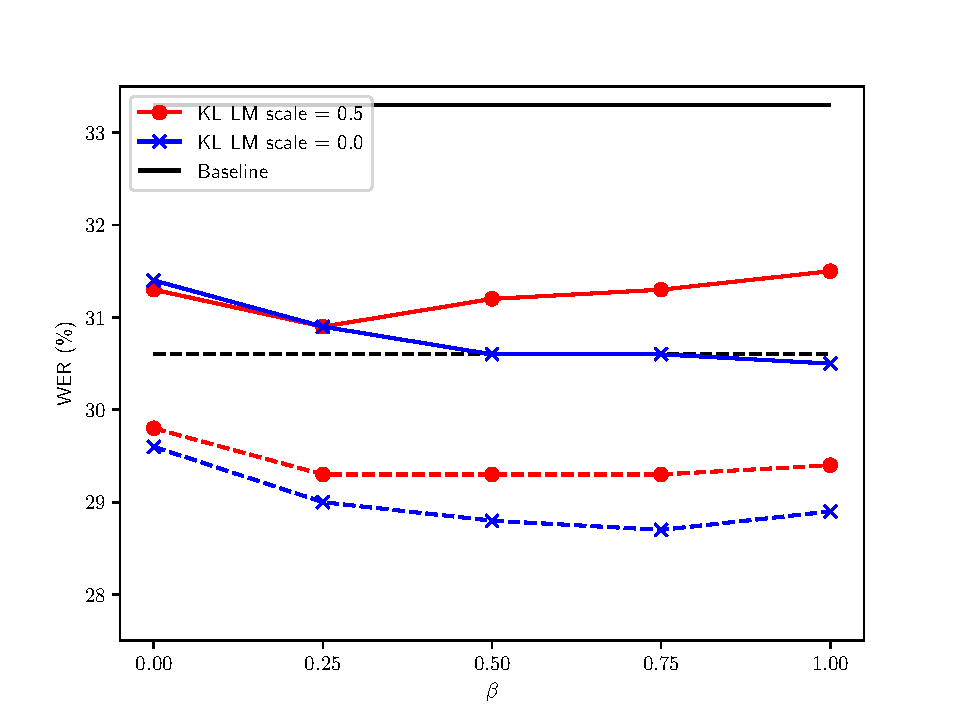
\includegraphics[width=\columnwidth]{figures/klfst_comparison}
%\end{figure}

For semi-supervised training, it is generally better to use a strong LM
for decoding unsupervised data to generate lattices.
From \cite{manohar2018semisup}, the best phone LM scale for interpolating 
normalization FST's phone LM scores and lattice's word LM scores 
when generating numerator supervision is 0.5.

In this section, we try to find:
\begin{enumerate}
  \item the best phone LM scale (0.0 vs 0.5) for interpolating phone LM and
    word LM scores to get numerator posteriors for the sequence-KL objective
  \item the best LM (3-gram vs 1-gram) to use for generating lattices to get
    numerator posteriors for sequence-KL
\end{enumerate}

The legend in Figure \ref{fig:lm_comparison} shows the LM used for decoding 
and the phone LM scale when generating supervision for sequence-KL objective. 
In the experiments in this section, we use the interpolated objective 
$(1-\beta)\Fmmi + \beta\Fkl$. 
Note that the LF-MMI objective in all cases uses a 3-gram word LM for decoding
and a phone LM scale of 0.5 for interpolating phone LM and word LM scores.

From Figure \ref{fig:lm_comparison}, when using a 3-gram word LM for 
decoding, using a phone LM scale of 0.0 (Blue $\times$) works better 
than a phone LM scale of 0.5 (Red $\circ$).
However, when using a 1-gram LM for decoding, the WER degrades with a phone LM
scale of 0.0 (Orange $*$) and gets even worse than baseline for large $\beta$.
This problem is alleviated if a phone LM scale of 0.5 is used (Green
$\triangle$), but is still worse than using 3-gram word LM for decoding.

From this, we conclude that for unsupervised domain adaptation, it is
better to use a strong LM like 3-gram for generating numerator supervision. 
This is also computationally advantageous
because using strong 3-gram LM requires only a single generation of lattices for
both MMI and sequence-KL, while using 1-gram LM requires regeneration of
lattices for sequence-KL.
Further, when using a strong word LM, interpolating the LM scores with 
phone LM scores is not required and using a phone LM scale of 0.0 works the
best.

The performance degradation when using a 
weak LM was also reported in \cite{kanda2017sequence-kl} for unsupervised
speaker adaptation. But we believe the degradation is larger in our case because
we are training the student network from scratch instead of initializing from
the teacher network. However, initializing from teacher network is not 
straight-forward in our case since the input features are different (16kHz vs
8kHz).

\begin{figure}[t]
  \centering
  \caption{\label{fig:lm_comparison} 8kHz Fisher  -\textgreater 16kHZ AMI-IHM
  WER(\%) results: Unigram vs 3-gram for sequence-KL. The solid lines show
results on {\em eval} and dashed lines on {\em dev}.}
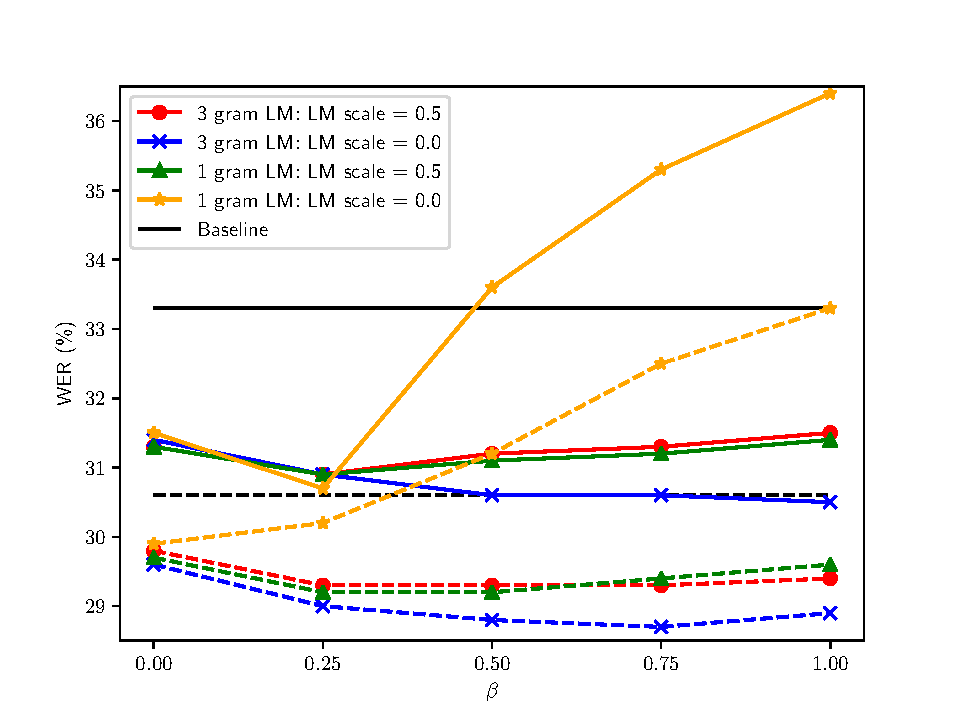
\includegraphics[width=\columnwidth]{figures/ug_comparison}
\end{figure}

\subsubsection{Multitask training for domain mismatch}

Multitask training is one of the methods for transfer learning in domain
mismatch conditions. In 
\cite{pegah2017transfer}, this was used for supervised adaptation. 
Here we apply it in the semi-supervised setting by
training on the Fisher data (upsampled to 16kHz) using LF-MMI and 
on the AMI-IHM data using an interpolated objective 
$(1-\beta)\Fmmi+\beta\Fkl$. Based on the results in Section
\ref{sec:lm_comparison}, we get numerator posteriors for sequence-KL 
from lattices obtained by decoding using a 3-gram Fisher word LM and 
using LM scores only from the word LM.
We share all the layers including the output for both Fisher and AMI tasks.
Figure \ref{fig:multilingual_comparison} compares the two for various
interpolation factors. We see that semi-supervised training in a
multitask approach (Red $\circ$) is better than training 
only on the unsupervised data (Blue $\times$) in the target domain, 
giving an improvement of around 3\% over
the ``Baseline''.  It is possible that training on a larger amount of data and
also regularizing with supervised Fisher data (even if out-of-domain) is helping
the cause here.  Since smaller $\beta$ is better, we can say LF-MMI is more
effective than using sequence-KL for multitask training in this domain mismatch
case. We believe that since the domains of the data used to train the teacher
and student networks are different (Fisher vs. AMI), the numerator posteriors
from the teacher are not very good for training the student using sequence-KL.
But, we can get better posteriors from the student network by training using
LF-MMI.

%\begin{table}[t]
%  \centering
%  \caption{\label{tab:bandwidth_results}WER(\%) results on AMI-IHM for 
%  domain adaptation from 8kHz Fisher to 16kHz AMI-IHM}
%  \begin{tabular}{l|lR{0.5cm} R{0.8cm} R{0.7cm}|cc}
%    System & LM & \multicolumn{3}{c|}{Target domain} & \multicolumn{2}{c}{WER(\%)} \\
%    & & sup (hrs) & unsup (hrs) & Rate (kHz) & dev & eval \\
%    \hline \hline
%    Baseline & -      & 0 & 0   & 8  & 30.6 & 33.3 \\
%    \hline
%    LF-MMI & Fisher & 0 & 80 & 16 & 30.3 & 31.5 \\
%    KL     & Fisher & 0 & 80 & 16 & 29.6 & 31.2 \\
%    LF-MMI & AMI    & 0 & 80 & 16 & 28.7 & 30.2 \\
%    KL     & AMI    & 0 & 80 & 16 & 28.8 & 30.2 \\
%    \hline
%    Wgt transfer    & AMI    & 0 & 80 &  8 & 27.2 & 28.8 \\
%    \hline
%    Oracle & -      & 80 & 0 & 16 & 18.7 & 18.6 \\
%    Oracle & -      & 80 & 0 & 8  & 20.4 & 19.9 \\
%    \hline
%  \end{tabular}
%\end{table}

\begin{figure}[t]
  \centering
  \caption{\label{fig:multilingual_comparison} 8kHz Fisher -\textgreater 16kHz
  AMI-IHM WER(\%) results: Unsupervised vs semi-supervised multitask training. 
The solid lines show results on {\em eval} and dashed lines on {\em dev}.}
  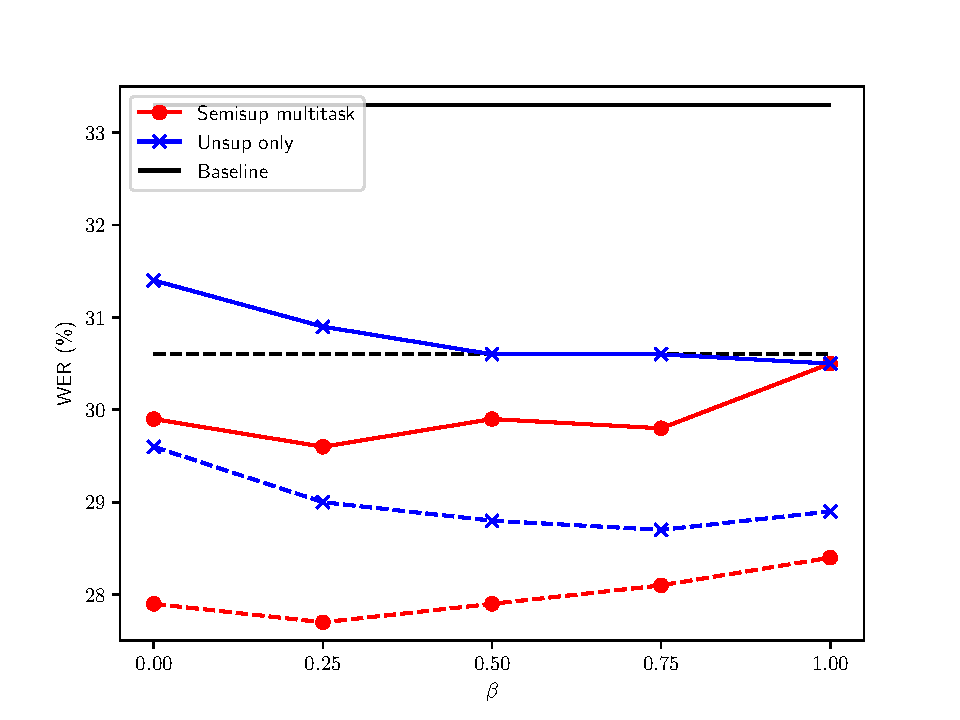
\includegraphics[width=\columnwidth]{figures/multilingual_comparison}
\end{figure}

%\begin{table}
%  \centering
%  \caption{\label{tab:interpolating_objectives} WER(\%) results interpolating 
%  LF-MMI and sequence-KL objectives for teacher-student learning. The
%interpolation weight on sequence-KL is $\beta$.}
%  \begin{tabular}{l|cc}
%    $\beta$ & dev & eval \\
%    \hline \hline
%    0 & 30.3 & 31.5 \\
%    0.1 & 30.0 & 31.2 \\
%    0.25 & 29.4 & 30.8 \\
%    0.5 & 29.0 & 30.4 \\
%    0.75 & 29.0 & 30.4 \\
%    1 & 29.6 & 31.2 \\
%    \hline
%  \end{tabular}
%\end{table}

\subsection{Headset to Distant microphone speech}

In this section, we report results on domain adaptation from AMI-IHM speech to AMI single distant microphone (SDM) speech.
For the baseline system, we use AMI-SDM data mixed with AMI-IHM data 
augmented with reverberation and noise. For supervision, we use lattices
generated from a GMM system for AMI-IHM data and use it for parallel
reverberated AMI-IHM data and AMI-SDM data as done in \cite{vijay_ami}.
%% Pegah: Does it mean that these experiments are semi-supervised and you use supervision for AMI-IHM?
For unsupervised domain adaptation experiments, we consider two unsupervised
dataset -- Mixer 6 \cite{mixer6-corpus} (We use only the telephone calls
portion) and ICSI \cite{icsi-corpus}. 
As teacher network, we use a TDNN-LSTM network trained on AMI-IHM data
that is mixed with reverberated and noise augmented version of the same. This
teacher network was selected as it gave the best performance on
AMI-IHM {\em dev} and {\em eval} sets. 
For adaptation using mixer 6, we decode the mixer 6 headset microphone
(MIC02) data using the teacher network
and a 3-gram Fisher word LM to generate
lattices. These lattices are converted into supervision for data from 
the parallel far-field microphones (MIC04-MIC13). Since the same data was 
recorded in multiple microphones, we only kept a subset of 30\% of the parallel
far-field data. 
For adaptation using ICSI, we decode the ICSI-IHM data using the teacher network
and the 3-gram AMI word LM to generate lattices. These lattices are converted 
into supervision for data from the parallel ICSI-SDM data. We used all 4
available distant microphones, but adjusted the training to train on these for
one-fourth the number of epochs as the rest of the data. In both the baseline
and T-S learning networks, we use the same i-vector extractor, 
which is trained on the same AMI data used to train the baseline. For both the
settings, we use semi-supervised training in a multitask approach
with supervised training with LF-MMI on the same AMI data as the baseline network
and unsupervised training with an interpolated objective
$(1-\beta)\Fmmi+\beta\Fkl$ on a mix of augmented (using reverberation and noise
addition) headset mic data and distant mic data from Mixer 6 or ICSI corpora.

The results in Table \ref{tab:sdm_results} show that T-S learning using 
parallel data in Mixer 6 or ICSI for adaptation from IHM to SDM improves the {\em dev} and {\em eval}
WERs  over the baseline, which uses only AMI. The hours column shows the amount (before augmentation) of 
supervised (AMI) and unsupervised (Mixer 6 or ICSI) data used. The improvement is found to be
larger when using ICSI corpus, probably because of the similarity of ICSI and
AMI corpora. 
%In the future, we will also do analysis using oracle experiments
%using ICSI.

\begin{table}[t]
  \centering
  \caption{\label{tab:sdm_results}IHM -\textgreater SDM adaptation: WER(\%) on
  AMI-SDM}
  \begin{tabular}{lc|rr|cc}
    Method & $\beta$ & \multicolumn{2}{c|}{Hours} & \multicolumn{2}{c}{WER(\%)} \\
    & & sup & unsup & {\em dev} & {\em eval}  \\
    \hline \hline
  Baseline & 0.0 & 80 & 0 & 34.0 & 37.2 \\
    \hline
    T-S (Mixer 6) & 0.5 & 80 & 110 & 33.7 & 37.0 \\
    T-S (ICSI) & 0.5 & 80 & 80 & 32.5 & 36.3 \\
    \hline
  \end{tabular}
\end{table}


%% Below is an example of how to insert images. Delete the ``\vspace'' line,
%% uncomment the preceding line ``\centerline...'' and replace ``imageX.ps''
%% with a suitable PostScript file name.
%% -------------------------------------------------------------------------
%\begin{figure}[htb]
%
%\begin{minipage}[b]{1.0\linewidth}
%  \centering
%  \centerline{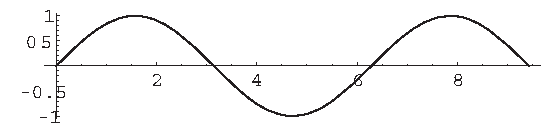
\includegraphics[width=8.5cm]{image1}}
%%  \vspace{2.0cm}
%  \centerline{(a) Result 1}\medskip
%\end{minipage}
%%
%\begin{minipage}[b]{.48\linewidth}
%  \centering
%  \centerline{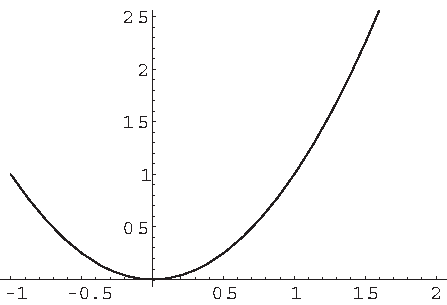
\includegraphics[width=4.0cm]{image3}}
%%  \vspace{1.5cm}
%  \centerline{(b) Results 3}\medskip
%\end{minipage}
%\hfill
%\begin{minipage}[b]{0.48\linewidth}
%  \centering
%  \centerline{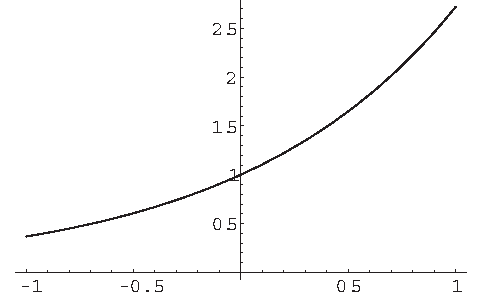
\includegraphics[width=4.0cm]{image4}}
%%  \vspace{1.5cm}
%  \centerline{(c) Result 4}\medskip
%\end{minipage}
%%
%\caption{Example of placing a figure with experimental results.}
%\label{fig:res}
%%
%\end{figure}

\section{Conclusions and Future work}
\label{sec:conclusions}
In this paper, we proposed a teacher-student learning approach for 
unsupervised domain adaptation of sequence-trained models. 
Here, we use a teacher network to decode the
unsupervised source-domain data to generate supervision. The supervision is used with
parallel data in the target-domain to train a student network.
We explored using lattice-free
MMI, sequence-KL divergence and an interpolation of the two objectives for training the student network. 
Based on our results on various domain adaptation scenarios, 
the recommended approach is to use semi-supervised multitask training with LF-MMI objective 
on the supervised portion of the data and 
an interpolation of LF-MMI and sequence-KL objectives on the unsupervised portion of the data. 
%An interpolation factor of 0.5 between the two objectives worked consistently for all cases.

In the scenario of {\em only} feature domain mismatch such as clean to noisy speech adaptation, 
parallel data is available in the source and target domains. 
In this scenario, we observed that sequence-KL is very
effective even when used for {\em purely} unsupervised training. 
However,  our recommended semi-supervised training approach 
gave significant WER improvement over this. 
In the scenario of mismatch in feature as well as language domains such as Fisher to AMI adaptation, we observed that LF-MMI objective is more helpful than sequence-KL.
For the sequence-KL objective, our proposed approach of using a strong LM for getting numerator
posteriors is better than using a weak LM in terms of WER. This is also computationally efficient since we reuse the supervision generated from the teacher network for LF-MMI, and pre-compute and dump the necessary numerator posteriors.


%We hypothesize that sequence-KL might be helpful in the beginning of training
%when initializing the network from scratch, and will try in the future to 
%vary the interpolation factor with LF-MMI as the training progresses.  
%In the future, we will also explore cases of adaptation using semi-supervised
%LF-MMI and sequence-KL for retraining the network without initializing from
%scratch. 
In the future, we will explore these ideas in the context of model
compression.

% To start a new column (but not a new page) and help balance the last-page
% column length use \vfill\pagebreak.
% -------------------------------------------------------------------------
\vfill
\pagebreak


% References should be produced using the bibtex program from suitable
% BiBTeX files (here: strings, refs, manuals). The IEEEbib.bst bibliography
% style file from IEEE produces unsorted bibliography list.
% -------------------------------------------------------------------------
\bibliographystyle{IEEEbib}
\bibliography{refs}

\end{document}
